\documentclass[12pt,a4paper]{article}
\usepackage{german}
\usepackage[utf8]{inputenc}
\usepackage[T1]{fontenc}
\usepackage{ae}
\usepackage{amssymb}
\usepackage{ifthen}
\ifx\pdfoutput\undefined
\usepackage[dvips]{graphicx}
\else
\usepackage[pdftex]{graphicx}
\pdfcompresslevel=9
\pdfpageheight=297mm
\pdfpagewidth=210mm
\usepackage{color}
\usepackage{hyperref}

\definecolor{uniblue}{rgb}{0, 0.2, 0.4}

\newcommand{\cmark}[1]{{\color{uniblue} \textbf{#1}}}


\hypersetup{
colorlinks=true,
pdfpagemode=UseNone,
pdfstartview=FitH,
pdfview=FitH,
urlcolor=uniblue,
linkcolor=uniblue
}
\fi
%%
\errorcontextlines=999
%
%
\def\hs#1{\hspace*{#1cm}}
\def\spiegel#1{$\stackrel{\leftarrow}{#1}$}
\def\mspiegel#1{\stackrel{\leftarrow}{#1}}
\def\ei#1{$\ \stackrel{(#1)}{=}\ $}
\def\mei#1{\ \stackrel{(#1)}{=}\ }
\def\als{~~~$\simeq$~~~}
\def\ab{$\stackrel{uses}{\longrightarrow}\ $}
%
%
\setlength{\textwidth}{175mm}
\setlength{\oddsidemargin}{0mm}
\setlength{\evensidemargin}{0mm}
\setlength{\topmargin}{0mm}
\setlength{\textheight}{252mm}
\setlength{\voffset}{-2.4cm}
\setlength{\hoffset}{-1.2cm}
\parskip1ex
\parindent0cm
%%
\def\rand#1{\marginpar{\tiny #1}}
\def\co#1{$\overline{\mbox{#1}}$}
\def\mco#1{\overline{\mbox{#1}}}         
\def\rhd{\vartriangleright}
\def\mouver{\vartriangleright\ }
\def\ouver{$\vartriangleright\ $}
\def\folgt{$\ \Longrightarrow\ $}
\def\gdw{$\ \Longleftrightarrow\ $}
\def\rhd{$\vartriangleright$}
\def\lhd{$\vartriangleleft$}
\def\brhd{$\blacktriangleright$}
\def\blhd{$\blacktriangleleft$}
\def\bst{$\bigstar$}
\def\ost{$\circledast$}
%%%
\def\err#1{$error_{#1}$}
\def\merr#1{error_{#1}}
%
\def\tsig{$T_{SIG}$}
%
\def\mt{$\times\ $}
\def\pot#1{{\Large $\wp$}(#1)}
\def\mpotf#1{{\Large \wp_{fin}}(#1)}
\def\ab{$\stackrel{uses}{\longrightarrow}\ $}
\def\wird{~{\tt ==>}~}
\def\move{~\vdash~}
\def\mv#1{~\stackrel{#1}{\vdash}~}
\def\moves{~\stackrel{*}{\vdash}~}
\def\movep{~\stackrel{+}{\vdash}~}
\def\regel{\ \longrightarrow\ }
\def\wirdm{\ \Longrightarrow\ }
\def\wirds{~\stackrel{*}{\Longrightarrow}~}
\def\alt{\ \vert\ }
%
%
\def\ww{{\tt \#t$\ $}}
\def\ff{{\tt \#f$\ $}}
\def\mww{\mbox{\tt \#t}}
\def\mff{\mbox{\tt \#f}}
%
\def\bool{I\hskip -1.6pt B$\ $}
\def\mbool{\rm I\hskip -1.6pt B}
%
\def\pot#1{{\Large $\wp$}(#1)}
\def\mrea{\rm I\hskip -1.6pt R}
\def\mnat{\rm I\hskip -1.6pt N}
\def\mnato{\rm I\hskip -1.6pt N_0}
\def\rea{I\hskip -1.6pt R$\ $}
\def\nat{I\hskip -1.6pt N$\ $}
\def\nato{I\hskip -1.6pt N_0$\ $}
\def\aus{$ \in\ $}
\def\bull{\vrule height .9ex width .8ex depth -.1ex }
\def\gdw{:$\Longleftrightarrow$}
\def\folgt{$\ \Longrightarrow\ $}
%
\def\se{$\ \bullet\ \ $}
\def\pa{$\ \parallel\ \ $}
\def\async{$\ \equiv\hskip -6pt\equiv\hskip -3pt\gg\ \ $}
\def\sync{$\ \bowtie\hskip -6pt\rhd\ \ $}
\def\nix{$\ \infty\ $}
\def\ka{$\cal K$}
\def\seperate{\hrule\vskip 2pt\hrule\vskip 2pt\hrule}
%
\def\seperate{\hrule\vskip 2pt\hrule\vskip 2pt\hrule}
%
\newcounter{beispiel}
\newenvironment{bsp}[2]{\label{#1}\addtocounter{beispiel}{1} \vskip 8pt
\seperate \vskip 6pt
{\bf Beispiel \thechapter.\thebeispiel:} ({\em #2}) \vskip -3pt }
{\vskip 6pt
\seperate \vskip 5pt}
%
\def\strich{\begin{center} \rule{7cm}{2pt} \end{center}}
%
\newenvironment{remark}{\begin{description}\item {\bf Bemerkung:} }
{ \end{description}}
%
% ***************************************************************
\def\eg#1{eg(#1)}
\def\ag#1{ag(#1)}
\def\bs{\vskip 0.7cm}
%
%
\newcommand{\bildw}[4]{
  \begin{figure}[htb]
    \begin{center}
      \includegraphics[width=#4 cm]{images/#2}
      \caption{#3}
      \label{#1}
    \end{center}
  \end{figure}
}
%
%
\newcommand{\bildh}[4]{
  \begin{figure}[hbt]
    \begin{center}
      \includegraphics[height=#4 cm]{images/#2}
      \caption{#3}
      \label{#1}
    \end{center}    
  \end{figure}
}
%
%
\newcommand{\bild}[3]{
  \begin{figure}[hbt]
    \begin{center}
      \includegraphics[width=\textwidth]{#2}
      \caption{#3}
      \label{#1}
    \end{center}    
 \end{figure}
}
%
%
\newcommand{\atitle}{
  \begin{center}
    \begin{minipage}[t]{16cm}
      \begin{minipage}{3cm}
        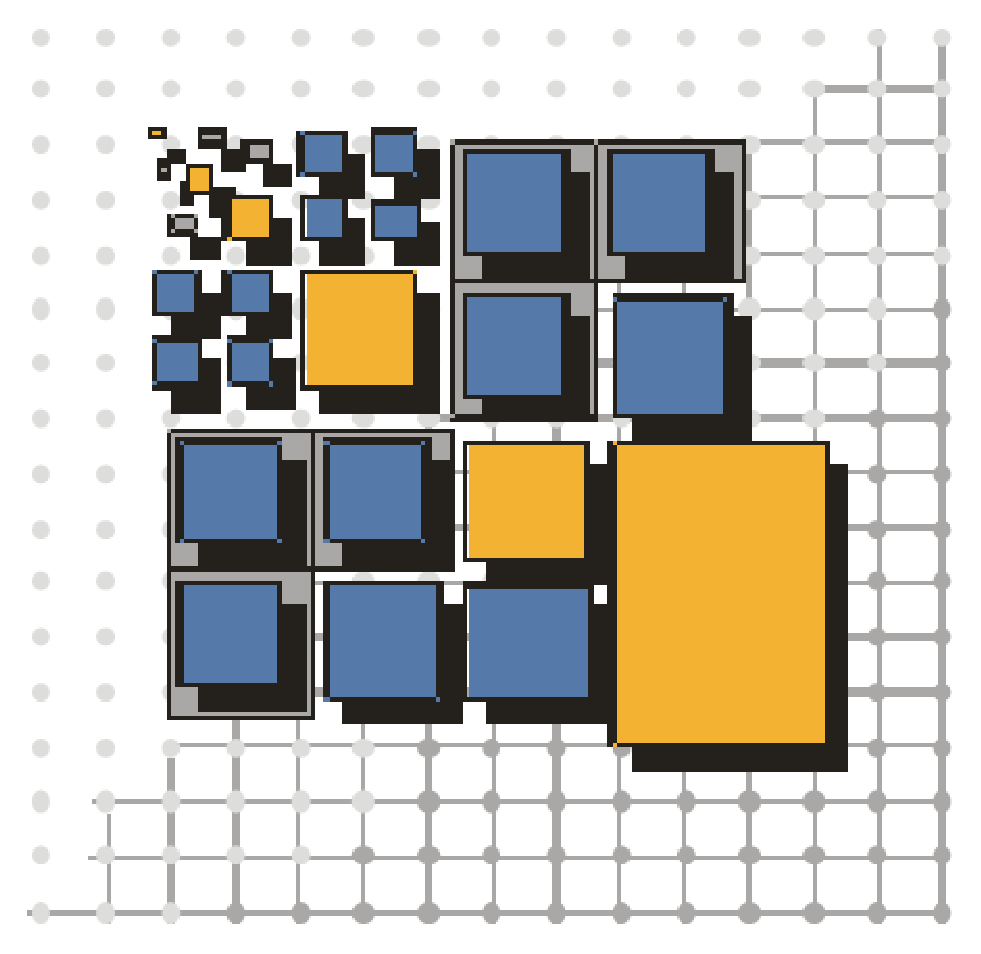
\includegraphics[height=26mm]{images/vs-logo}
      \end{minipage}
      \hfill
      \begin{minipage}{9cm}
        \centering
        {\small Otto-Friedrich-Universität Bamberg\\}
        {\Large Lehrstuhl für Praktische Informatik\\}
			 \vspace{0.3cm}
      \end{minipage}
      \hfill
      \begin{minipage}{3cm}
        
\includegraphics[height=26mm]{images/uni}
      \end{minipage}
    \end{minipage}\\[7ex]
  \end{center}
  \ifx\pdfoutput\undefined
  \else
  \hypersetup{
    pdfauthor={Distributed Systems Group},
    pdfsubject={Richtlinien zur Erstellung von Seminar- und Abschlussarbeiten},
    pdftitle={Richtlinien zur Erstellung von Seminar- und Abschlussarbeiten}
  }
  \fi
}
%
%
\newcommand{\cci}{\\[-6ex]}
\newcommand{\cc}{\\[-4.5ex]}
%
%
\newcounter{LAufgabe}
\newenvironment{LAufgabe}{
  \addtocounter{LAufgabe}{
    \large\sc L\"osungsvorschlag  zu Aufgabe
    \theLAufgabe\\[1ex]
  }
}
{\vspace{0.5ex}}
%
%
\newcounter{Aufgabe}
\newenvironment{Aufgabe}{
  \addtocounter{Aufgabe}{1}{
%    \large\sc Aufgabe \theAufgabe\\[1ex]
  }
}
{\vspace{0.5ex}}
%
%
\newcommand{\No}{\N_0}
\newcommand{\N}{\mathbb{N}}
\newcommand{\R}{\mathbb{R}}
\newcommand{\Z}{\mathbb{Z}}
\newcommand{\Q}{\mathbb{Q}}
%
\newcommand{\Ltitel}[1]{
{~\\[-2.5cm] 
\begin{center}
\Large\sc Informatik I~$\cdot$~
{\LARGE\sc \"Ubungsblatt #1}~$\cdot$~WiSe 1997/98
\end{center}~\\[-52pt]}{\LARGE\sc
~\begin{center}
L\"osungsvorschl\"age\\[4ex]
\end{center}
}}
%
%
\newcommand{\link}[2]{
  \ifx\pdfoutput\undefined
  #1 (#2)
  \else
  \href{#2}{#1}
  \fi  
}

%%% Local Variables: 
%%% mode: latex
%%% TeX-master: "ueb1"
%%% TeX-master: t
%%% TeX-master: t
%%% End: 
